\noindent
\begin{minipage}[t]{125pt}
  \vspace*{73pt}
  \noindent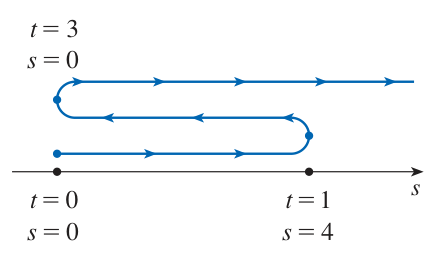
\includegraphics[width=\linewidth]{images/p0262_fig1.png}
  \vspace{5pt}

  \noindent{\small\textsf{\textbf{HÌNH 2}}}

  \vspace{74pt}
  \noindent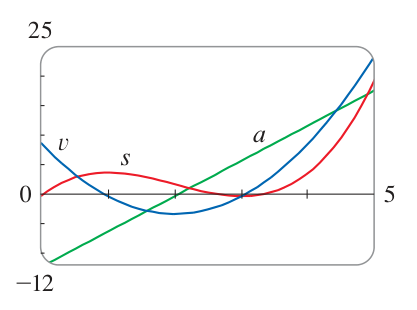
\includegraphics[width=\linewidth]{images/p0262_fig2.png}
  \vspace{7pt}

  \noindent{\small\textsf{\textbf{HÌNH 3}}}

  \vspace{266pt}
  \noindent{\small\textsf{\textbf{HÌNH 4}}}
\end{minipage}%
\hspace{25pt}%
\begin{minipage}[t]{390pt}
  \setlength{\parskip}{4.5pt}
  \setlength{\abovedisplayskip}{3pt}
  \setlength{\belowdisplayskip}{3pt}

  Bất đẳng thức này đúng khi cả hai thừa số đều dương ($t > 3$) hoặc khi cả hai thừa số đều âm ($t < 1$). Do đó chất điểm chuyển động theo chiều dương trong các khoảng thời gian $t < 1$ và $t > 3$. Nó chuyển động lùi (theo chiều âm) khi $1 < t < 3$.

  \textbf{(e)}\enspace Sử dụng thông tin từ phần (d), chúng ta vẽ một sơ đồ phác thảo trong Hình~2 về chuyển động qua lại của chất điểm dọc theo một đường thẳng (trục $s$).

  \textbf{(f)}\enspace Do những gì đã tìm hiểu ở các phần (d) và (e), chúng ta cần tính riêng quãng đường đi được trong các khoảng thời gian $[0, 1]$, $[1, 3]$ và $[3, 5]$.

  Quãng đường đi được trong giây đầu tiên là
  \[
  |f(1) - f(0)| = |4 - 0| = 4\text{ m}
  \]
  Từ $t = 1$ đến $t = 3$, quãng đường đi được là
  \[
  |f(3) - f(1)| = |0 - 4| = 4\text{ m}
  \]
  Từ $t = 3$ đến $t = 5$, quãng đường đi được là
  \[
  |f(5) - f(3)| = |20 - 0| = 20\text{ m}
  \]
  Tổng quãng đường là $4 + 4 + 20 = 28\text{ m}$.

  \textbf{(g)}\enspace Gia tốc là đạo hàm của hàm vận tốc:
  \[
  a(t) = \frac{d^2s}{dt^2} = \frac{dv}{dt} = 6t - 12
  \]
  \[
  a(4) = 6(4) - 12 = 12\text{ m/s}^2
  \]

  \textbf{(h)}\enspace Hình~3 thể hiện các đồ thị của $s$, $v$ và $a$.

  \textbf{(i)}\enspace Chất điểm tăng tốc khi vận tốc dương và tăng ($v$ và $a$ đều dương) và cả khi vận tốc âm và giảm ($v$ và $a$ đều âm). Nói cách khác, chất điểm tăng tốc khi vận tốc và gia tốc cùng dấu. (Chất điểm bị đẩy theo cùng hướng nó đang chuyển động.) Từ Hình~3, ta thấy điều này xảy ra khi $1 < t < 2$ và khi $t > 3$. Chất điểm giảm tốc khi $v$ và $a$ trái dấu, tức là khi $0 \le t < 1$ và khi $2 < t < 3$. Hình~4 tóm tắt chuyển động của chất điểm.

  \vspace{6pt}
  \begin{center}
    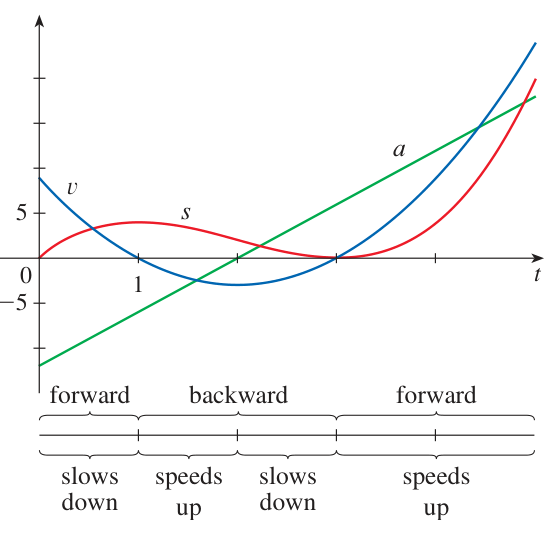
\includegraphics[width=0.92\linewidth]{images/p0262_fig3.png}
  \end{center}
  \vspace{-10pt}
  \hfill\textcolor{stewartblue}{\rule{1.2ex}{1.2ex}}
\end{minipage}
